\chapter{Munich WAN}

\section{Site Overview}
Munich is the other branch of the RECOMP Corporation. The network has:
\begin{itemize}
    \item Two Routers (2911 model);
    \item Four switch Layer 2 switches (2960-24TT model);
    \item Four PCs representing each of the networks present in each branch: Staff, Accounting, Human Resources and Users.
\end{itemize}

The topology of the Munich branch is shown in Figure \ref{fig:munichtopology}. The Munich \ac{WAN} is connected to the Internet using the address block 193.136.60.147/29.

\begin{figure}[!htb]
\centering
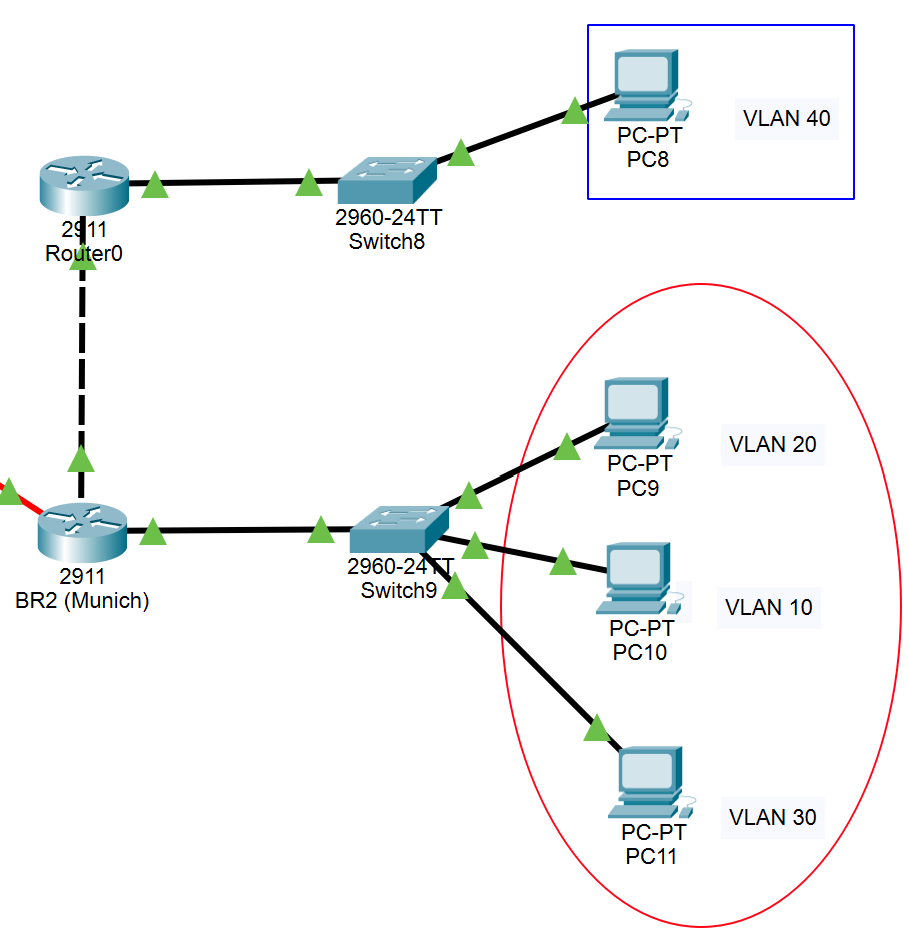
\includegraphics[width=0.6\textwidth]{figures/munich_topology.png}
\caption{\label{fig:munichtopology}Munich WAN Topology}
\end{figure}


\section{Munich Subnet Implementation}

In this subchapter, you will find the addressing for this branch in Table \ref{tab:munich-addressing}. This branch, like the previous one, contains four VLANs, each with a number of nodes, a network address, a broadcast address, a mask, and a range of addresses that can be used for each machine on the network.

\begin{table}[h]
\centering
\resizebox{\textwidth}{!}{%
\begin{tabular}{lccccc}
\hline
\textbf{Network} & \textbf{Number of Nodes} & \textbf{Network Address} & \textbf{Broadcast Address} & \textbf{Mask} & \textbf{First--Last Valid Address} \\
\hline
USERS & 200 & 172.18.78.0 & 172.18.78.255 & /24 & 172.18.78.1 -- 172.18.78.254 \\
ACCOUNTING & 20 & 172.18.79.0 & 172.18.79.31 & /27 & 172.18.79.1 -- 172.18.79.30 \\
STAFF & 10 & 172.18.79.32 & 172.18.79.47 & /28 & 172.18.79.33 -- 172.18.79.46 \\
HR & 10 & 172.18.79.48 & 172.18.79.63 & /28 & 172.18.79.49 -- 172.18.79.62 \\
\hline
\end{tabular}%
}
\caption{Munich \ac{WAN} \ac{IP} addressing scheme}
\label{tab:munich-addressing}
\end{table}


As shown in Figure \ref{fig:munichaddressing}, the addressing for the Munich branch is presented.

\begin{figure}[!htb]
\centering
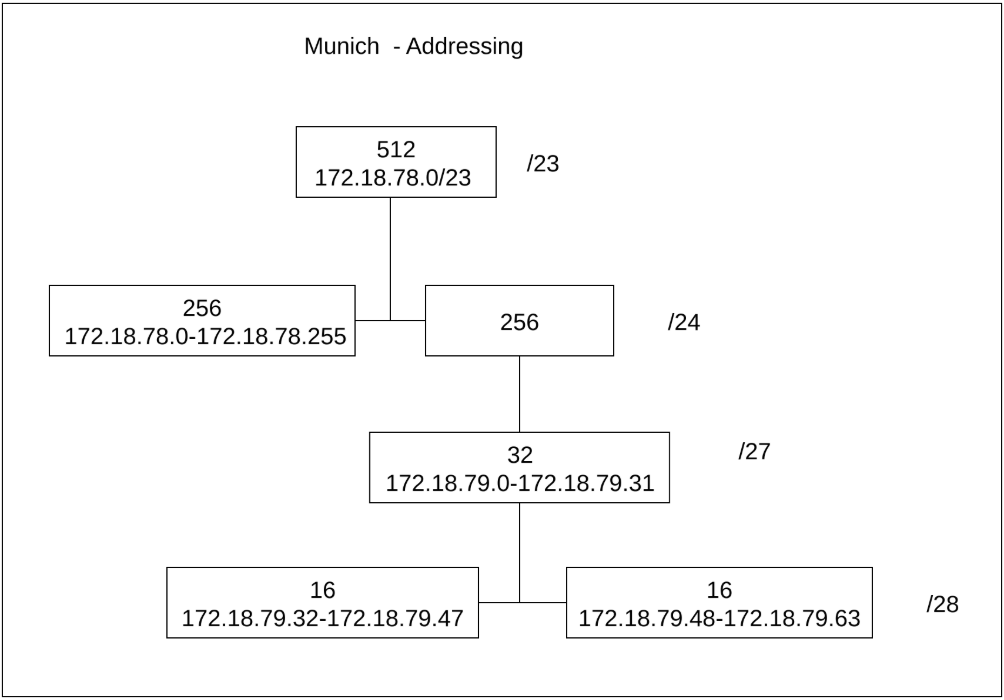
\includegraphics[width=0.6\textwidth]{figures/munich_addressing.png}
\caption{\label{fig:munichaddressing}Munich IP Addressing}
\end{figure}

\section{Implementation of Cisco Commands}

In this Munich branch, the goal was to implement VLAN segmentation, inter-VLAN routing, DHCP address allocation and connectivity between remote sites through static routing.

\subsection*{Switch Configuration}

The Switch7 (SW7), was configured to handle three departments: Staff, Accounting, and Human Resources (HR).
The following VLANs were created:

\begin{lstlisting}[caption={VLAN creation on SW7}, label={lst:sw7-vlan-creation}]
vlan 10
  name STAFF
vlan 20
  name ACCOUNTING
vlan 30
  name HR
vlan 50
  name NATIVE
vlan 99
  name BLACKHOLE
\end{lstlisting}

The trunk link connecting SW7 to router BR2 was configured on the \textit{gigabitEthernet0/1} interface, allowing VLANs 10, 20 and 30 and using VLAN 50 as the native VLAN:

\begin{lstlisting}[caption={Trunk configuration on SW7}, label={lst:sw7-trunk}]
interface gigabitEthernet0/1
    switchport mode trunk
    switchport trunk native vlan 50
    switchport trunk allowed vlan 10,20,30
\end{lstlisting}

The access ports for the end-user PCs were then assigned to their respective VLANs.

\begin{lstlisting}[caption={Access port configuration on SW7}, label={lst:sw7-access}]
interface range fa0/1-5
    switchport mode access
    switchport access vlan 10
    no shutdown
exit

interface range fa0/6-10
    switchport mode access
    switchport access vlan 20
    no shutdown
exit

interface range fa0/11-15
    switchport mode access
    switchport access vlan 30
    no shutdown
exit

interface range fa0/16-24
    switchport mode access
    switchport access vlan 99
    shutdown
\end{lstlisting}

The ports not used were assigned to Blackhole VLAN 99 and administratively shutdown to improve security.

Switch8 (SW8), used for local users in Users VLAN 40, was configured with VLAN 40, 50 and 99:

\begin{lstlisting}[caption={VLAN creation on SW8}, label={lst:sw8-vlan-creation}]
vlan 40
  name USERS
vlan 50
  name NATIVE
vlan 99
  name BLACKHOLE
\end{lstlisting}


Secondly, we configured many different network interfaces for vlan 40 and vlan 99:

\begin{lstlisting}[caption={Access port configuration on SW8}, label={lst:sw8-access}]
interface range fa0/1-24
    switchport mode access
    switchport access vlan 40
    no shutdown
exit

interface range gigabitEthernet0/2
    switchport mode access
    switchport access vlan 99
    shutdown
exit    
\end{lstlisting}

\subsection{Router Configuration}
This subsection demonstrates the configuration of two routers: BR2 and Router0 (R0).
\vspace{0.1cm}
\subsubsection*{BR2}

The BR2 router is connected to the internet with the IP address 193.136.60.147/29. The R0 router is connected to the BR2 router with a crossover cable.

First, the gigabitEthernet0/0 interface was configured, connecting the BR2 router to the internet. Therefore, we have the following code:

\begin{lstlisting}[caption={Interface GigabitEthernet0/0 Configuration}, label={lst:intf-gb0/0}]
interface gigabitEthernet0/0
  ip address 193.136.60.147 255.255.255.248
  no shutdown
exit
\end{lstlisting}

On the BR2 router, four subinterfaces were configured to handle traffic from different VLANs over a single physical interface. Each subinterface is identified by a \texttt{.} followed by the VLAN number, which allows the router to distinguish between the different VLANs. The command \texttt{encapsulation dot1q <VLAN>} specifies that 802.1Q trunking is being used, enabling the physical interface to carry traffic from multiple VLANs simultaneously.

The IP addresses assigned to each subinterface allow the router to act as the default gateway for the hosts in the corresponding VLANs:

\begin{itemize}
    \item GigabitEthernet0/1.10: configured for VLAN 10 with IP address \texttt{172.18.79.46/28}. This subinterface provides routing and inter-VLAN connectivity for devices in VLAN 10.
    \item GigabitEthernet0/1.20: configured for VLAN 20 with IP address \texttt{172.18.79.30/27}, serving as the gateway for devices in VLAN 20.
    \item GigabitEthernet0/1.30: configured for VLAN 30 with IP address \texttt{172.18.79.62/28}, providing routing services for VLAN 30 hosts.
    \item GigabitEthernet0/1.50: configured for VLAN 50 as the native VLAN. No IP address is assigned because this VLAN is likely used only for untagged traffic passing through the trunk, without requiring routing.
\end{itemize}

By assigning unique IP addresses to each subinterface, the router can perform inter-VLAN routing, allowing devices on different VLANs to communicate while still maintaining VLAN segmentation. This setup efficiently leverages a single physical interface to carry multiple networks, reducing hardware requirements and simplifying the network topology.

\begin{lstlisting}[caption={Subinterfaces configuration on BR2 router}, label={lst:subintf-BR2}]
interface gigabitEthernet0/1.10
  encapsulation dot1q 10
  ip address 172.18.79.46 255.255.255.240

interface gigabitEthernet0/1.20
  encapsulation dot1q 20
  ip address 172.18.79.30 255.255.255.224

interface gigabitEthernet0/1.30
  encapsulation dot1q 30
  ip address 172.18.79.62 255.255.255.240

interface gigabitEthernet0/1.50
  encapsulation dot1q 50 native
  no ip address
\end{lstlisting}


Next, using the \textit{no shutdown} command, the interface connecting BR2 to SW7 was enabled.

\begin{lstlisting}[caption={Turn on Interface GigabitEthernet0/1 between SW7 and BR2}, label={lst:sw7-BR2}]
interface gigabitEthernet0/1
  no shutdown
exit
\end{lstlisting}

\vspace{0.1cm}
\subsubsection*{R0}

Router R0 is connected to a switch, and that switch has only one associated VLAN, that's VLAN 40, which is USERS. 
First, the GigabitEthernet0/0 interface was configured to connect router BR2 to router R0 with the IP address 193.136.60.148/29 on R0 side.

\begin{lstlisting}[caption={Interface GigabitEthernet0/0 configuration on R0}, label={lst:r0-br2connection}]
interface gigabitEthernet0/0
  ip address 193.136.60.148 255.255.255.248
  no shutdown
exit
\end{lstlisting}

Next, the interface connecting R0 to SW8 was configured. The IP address assigned in the configuration of this interface was 172.18.78.254/24.
\begin{lstlisting}[caption={Configuring the GigabitEthernet0/1 interface on R0}, label={lst:r0-if_gb0/0}]
interface gigabitEthernet0/1
  ip address 172.18.78.254 255.255.255.0
  no shutdown
exit
\end{lstlisting}


\subsection{DHCP Configuration}
In this subchapter, we will explain the DHCP configuration on the two Munich WAN routers for the VLANs of each of the two switches in this network.
DHCP, basically, is a protocol that automatically assigns IP addresses and other network settings, (for example: gateway, DNS) to devices on a network.

\vspace{0.1cm}
\subsubsection*{BR2 Router}
On the BR2 router, three DHCP pools were configured, corresponding to the VLANs connected to the SW7 switch: VLAN 20 (STAFF), VLAN 10 (ACCOUNTING), and VLAN 30 (HR).  
Each pool defines a specific IP range, the respective default gateway, DNS server, and same domain name to be distributed to the hosts within that VLAN. Additionally, several IP addresses were excluded to prevent them from being assigned dynamically—typically reserved for network devices such as routers and switches.

\begin{lstlisting}[caption={Exclusion of static addresses already defined to avoid errors}, label={lst:errors}]
ip dhcp excluded-address 172.18.79.33 172.18.79.45
ip dhcp excluded-address 172.18.79.1 172.18.79.29
ip dhcp excluded-address 172.18.79.49 172.18.79.61
\end{lstlisting}

\begin{lstlisting}[caption={Creation of a DHCP pool called STAFF}, label={lst:staff-pool}]
ip dhcp pool STAFF
 network 172.18.79.32 255.255.255.240
 default-router 172.18.79.46
 dns-server 8.8.8.8
 domain-name RECOMP2526M1A06.recomp.com 
exit
\end{lstlisting}

\begin{lstlisting}[caption={Creation of a DHCP pool called ACCOUNTING}, label={lst:ACCOUNTING-pool}]
ip dhcp pool ACCOUNTING
 network 172.18.79.0 255.255.255.224
 default-router 172.18.79.30
 dns-server 8.8.8.8
 domain-name RECOMP2526M1A06.recomp.com
exit
\end{lstlisting}

\begin{lstlisting}[caption={Creation of a DHCP pool called HR}, label={lst:HR-pool}]
ip dhcp pool HR
 network 172.18.79.48 255.255.255.240
 default-router 172.18.79.62
 dns-server 8.8.8.8
 domain-name RECOMP2526M1A06.recomp.com
exit
\end{lstlisting}

This configuration ensures that each VLAN has its own DHCP scope, allowing devices in each network to automatically obtain an IP address, gateway, and DNS information corresponding to their VLAN. 


The use of excluded address ranges guarantees that static IPs assigned to infrastructure components will not conflict with dynamically assigned addresses.
It should be noted that this DHCP configuration in Packet Tracer will have significant positive effects on PC9 (Vlan 20), PC10 (Vlan 10) and PC11 (Vlan 30).

\newpage
For example, if you look at the DHCP settings on PC9 in the following figure \ref{fig:munich_pc9}, you will see that it corresponds to Code \ref{lst:staff-pool} and that it contains exactly the assigned DNS IP (Google) and the corresponding default-gateway from the Staff Pool.

\begin{figure}[!h]
\centering
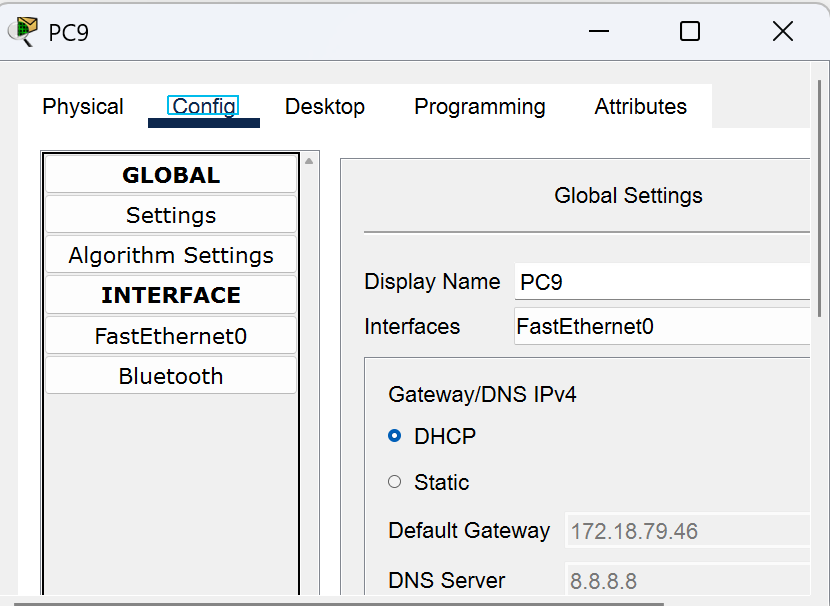
\includegraphics[width=0.5\textwidth]{figures/pc9_conf_example.png}
\caption{\label{fig:munich_pc9}Demonstration of PC9 DNS and your Default-Gateway}
\end{figure}

\subsection{IP Route Configuration}

In this subsection, the configuration of IP routes in packet tracer on router BR2, as well as on router R0, is demonstrated. 
\vspace{0.1cm}
\subsubsection*{BR2}

\begin{lstlisting}[caption={IP Route Demonstration of BR2 Router}, label={lst:br2router_iproute}]
ip route 172.18.78.0 255.255.255.0 193.136.60.148
\end{lstlisting}

In the Code \ref{lst:br2router_iproute}, it can be seen that there is an IP designated by \textit{172.18.78.0} which is the network address of router R0, followed by the network mask /24, and finally there is the IP address \textit{193.136.60.148} which is the IP of the next-hop or the IP of the neighboring router, i.e. is, the IP of Router0 where the traffic will be sent and reach the destination network.

\vspace{0.1cm}
\subsubsection*{R0}
In this subsection, the configuration of static IP routes in Packet Tracer on Router0 is presented. 

\begin{lstlisting}[caption={IP Route Demonstration of Router0}, label={lst:router0_iproute}]
ip route 172.18.79.0 255.255.255.224 193.136.60.147
ip route 172.18.79.32 255.255.255.240 193.136.60.147
ip route 172.18.79.48 255.255.255.240 193.136.60.147
\end{lstlisting}

In the Code \ref{lst:router0_iproute}, it can be observed that three static routes are configured on Router0. The first route defines the network \textit{172.18.79.0/27}, the second route defines the network \textit{172.18.79.32/28}, and the third route defines the network \textit{172.18.79.48/28}. All these networks are reachable through the next-hop IP address \textit{193.136.60.147}, which corresponds to the neighboring router BR2. 

Therefore, these static routes allow Router0 to forward traffic destined for the mentioned networks through BR2, ensuring proper communication between the subnets and the rest of the topology.
